\documentclass{ieeeaccess}
\usepackage{cite}
\usepackage{amsmath,amssymb,amsfonts}
\usepackage{algorithmic}
\usepackage{graphicx}
\usepackage{textcomp}
\usepackage{threeparttable}

\usepackage{bm}
\makeatletter
\AtBeginDocument{\DeclareMathVersion{bold}
\SetSymbolFont{operators}{bold}{T1}{times}{b}{n}
\SetSymbolFont{NewLetters}{bold}{T1}{times}{b}{it}
\SetMathAlphabet{\mathrm}{bold}{T1}{times}{b}{n}
\SetMathAlphabet{\mathit}{bold}{T1}{times}{b}{it}
\SetMathAlphabet{\mathbf}{bold}{T1}{times}{b}{n}
\SetMathAlphabet{\mathtt}{bold}{OT1}{pcr}{b}{n}
\SetSymbolFont{symbols}{bold}{OMS}{cmsy}{b}{n}
\renewcommand\boldmath{\@nomath\boldmath\mathversion{bold}}}
\makeatother

\graphicspath{{.}}

\def\BibTeX{{\rm B\kern-.05em{\sc i\kern-.025em b}\kern-.08em
    T\kern-.1667em\lower.7ex\hbox{E}\kern-.125emX}}

%Your document starts from here ___________________________________________________
\begin{document}
\history{Date of publication xxxx 00, 0000, date of current version xxxx 00, 0000.}
\doi{10.1109/ACCESS.2024.0429000}

\title{Increasing the Strength of Pervious Concrete While Maintaining 
       its Permability}
\author{
    \uppercase{Pranav V}\authorrefmark{1}, \uppercase{Abhay V}\authorrefmark{1}, 
    \uppercase{Suyash J}\authorrefmark{1}, \uppercase{Soham S}\authorrefmark{2},
    \uppercase{Rakshith P}\authorrefmark{3}
}

\address[1]{Department of Electronics and Communication Engineering,
            RV College of Engineering, Bangalore, India}
\address[1]{Department of Mechanical Engineering,
            RV College of Engineering, Bangalore, India}
\address[1]{Department of Information Science and Engineering,
            RV College of Engineering, Bangalore, India}

\markboth
{Author \headeretal: Preparation of Papers for IEEE TRANSACTIONS and JOURNALS}
{Author \headeretal: Preparation of Papers for IEEE TRANSACTIONS and JOURNALS}

\corresp{Corresponding author: Pranav V (e-mail: pranavvv.ec24@rvce.edu.in).}


\begin{abstract}
Pervious concrete is a sustainable construction material developed to mitigate
urban issues such as stormwater runoff, reduced groundwater recharge, and
surface flooding. This study focuses on the design and experimental
evaluation of a pervious concrete mix aimed at achieving adequate
mechanical strength while ensuring desirable permeability. The
investigation involved selecting suitable aggregates, determining an
appropriate water–cement ratio, and incorporating admixtures to enhance
overall performance. Compressive strength, tensile strength, and
permeability tests were conducted to assess the mix’s applicability in
pavements and low-traffic areas. The results demonstrated that the proposed
mix design offers a practical balance between structural integrity and
permeability, highlighting its potential as an environmentally friendly
alternative to conventional paving materials. Additionally, the paper
discusses challenges encountered during mix design and implementation and
suggests directions for future research to enable its effective use in
large-scale applications.
\end{abstract}

\begin{keywords}
    Pervious concrete, Sustainable Engineering, 
\end{keywords}

\titlepgskip=-21pt

\maketitle

\section{Introduction}
\label{sec:introduction}
\PARstart{R}{apid} urbanization has led to extensive construction of impervious 
surfaces such as asphalt and conventional concrete pavements, which disrupt the 
natural hydrological cycle. These surfaces prevent water infiltration, resulting 
in increased surface runoff, urban flooding, and reduced groundwater recharge. 
In response to these environmental concerns, there has been a growing interest 
in sustainable construction materials that support stormwater management. One 
such material is pervious concrete, a special type of concrete with a high void 
content that allows water to pass through its structure. 

Pervious concrete is composed of coarse aggregates, cement, water, and little to 
no fine aggregates. Its interconnected pore network enables infiltration of 
rainwater, making it suitable for sidewalks, parking lots, driveways, and 
low-traffic roads. In addition to hydrological benefits, pervious concrete can 
reduce the urban heat island effect, improve skid resistance, and contribute 
toward LEED (Leadership in Energy and Environmental Design) credits in green 
building certification systems. 

Despite its advantages, the widespread use of pervious concrete has been limited 
due to challenges in achieving an optimal balance between permeability and 
mechanical strength. In this study, we focus on the effects of the  water-cement 
ratio on the physical properties of pervious concrete. To this end, two batches 
of 6 pervious concrete cylinders, with the second batch having a lower 
water-cement ratio, were made, and tested for compresssive strength, split 
tensile strength, and permeability. Superplasticizer (SP) was used to increase 
the workability of the mixes made with the second recipe. 



\section{Experimental Setup}
Two batches of 6 cylinders each were cast. Common to both batches were the
cementitious material which was a mixture of cement and fly-ash in the ratio of 
4:1 by mass, coarse aggregates whose sizes ranged from 4.75-9.5 mm, 
and polypropylene fibres (PPF). 
\
\begin{table}
    \begin{threeparttable}
        \caption{\textbf{Mix Design}}
        \label{table:mix-design}
        \setlength{\tabcolsep}{20pt}
        \def\arraystretch{1.5}%
        \begin{tabular}{ l r  r }
            \hline
            & \multicolumn{1}{c}{Batch 1} & \multicolumn{1}{c}{Batch 2} \\
            \hline
            Cement, $kg/m\textsuperscript{3}$  & 280  & 280  \\
            Coarse Aggregate, $kg/m\textsuperscript{3}$ & 1420 & 1420 \\
            Fly-ash, $kg/m\textsuperscript{3}$ & 70   & 70   \\
            Water, $kg/m\textsuperscript{3}$   & 119  & 95.2 \\
            SP, $\%$\textsuperscript{1}        & ---  & 0.5  \\
            PPF, $\%$\textsuperscript{2}       & 0.2  & 0.2  \\
            \hline
        \end{tabular} 
        \begin{tablenotes}
            \item[1] \footnotesize of cementitious material
            \item[2] \footnotesize of aggregates
        \end{tablenotes}
    \end{threeparttable}
\end{table}
\
The proportions for the rest of the materials used are given in table 
\ref{table:mix-design}.

\section{Testing Method}
The samples were tested after 14 and 28 days for its tensile strength, its
compressive strength, and for its permeability.

\subsection{Compressive Strength}
The sample was placed in the universal testing machine (UTM) on one of its 
circular faces, and compressed. The pace rate was set to 1.8 KN/s. 
The compressive strength $f_c$ is calculated with the formula 
\[f_c = \frac{P}{A}\] where $P$ is the maximum force on the sample, and $A$ is
the area over which the force is applied.

\subsection{Tensile Strength}
The tensile strength was found using the Brazilian test, in which, the sample
was placed horizontally, in between two metal bars oriented parallel to the axis
of the sample, inside the UTM. The tensile strength $f_t$ was calculated with
the formula \[f_t = \frac{2P}{\pi LD}\] where $P$ is the force at the point of
failure, and $L$ and $D$ are respectively the length and the diameter of the
sample.

\subsection{Permeability}
The tensile strength was found using a makeshift falling head permeameter.
By measuring the time taken for the head to move from a height $h_1$ down to
$h_2$, the coefficient of permeability $k$ (in $mm/s$) can be calculated using
the formula \[k = \frac{aL}{At} \ln{\frac{h_1}{h_2}}\] where $a$ is the
cross-sectional area of the standpipe, $t$ is the time taken for the head to
fall from $h_1$ to $h_2$, and $L$ and $A$ are the dimensions of the sample.

\begin{figure}[h]
    \caption{Sample being tested for tensile strength}
    \centering
    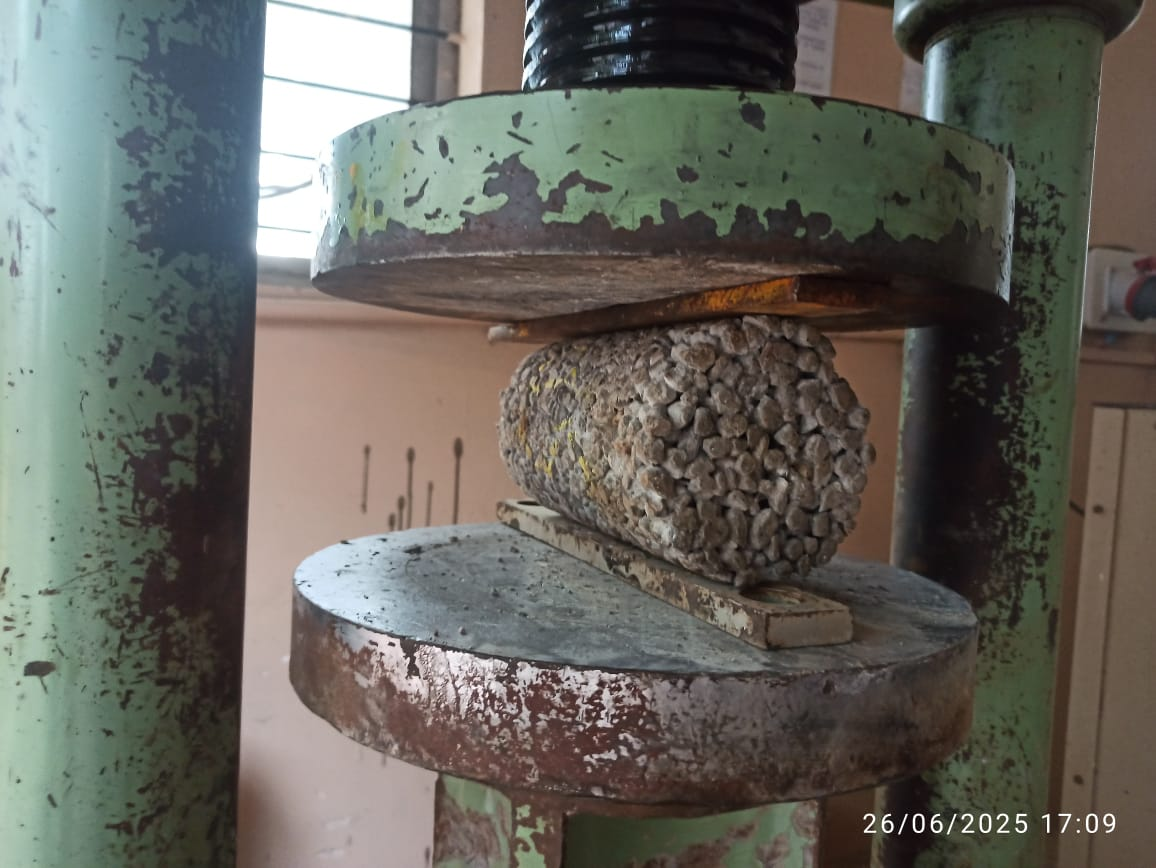
\includegraphics[scale=0.15]{tensile}
\end{figure}

\begin{figure}[h]
    \caption{Sample being tested for compressive strength}
    \centering
    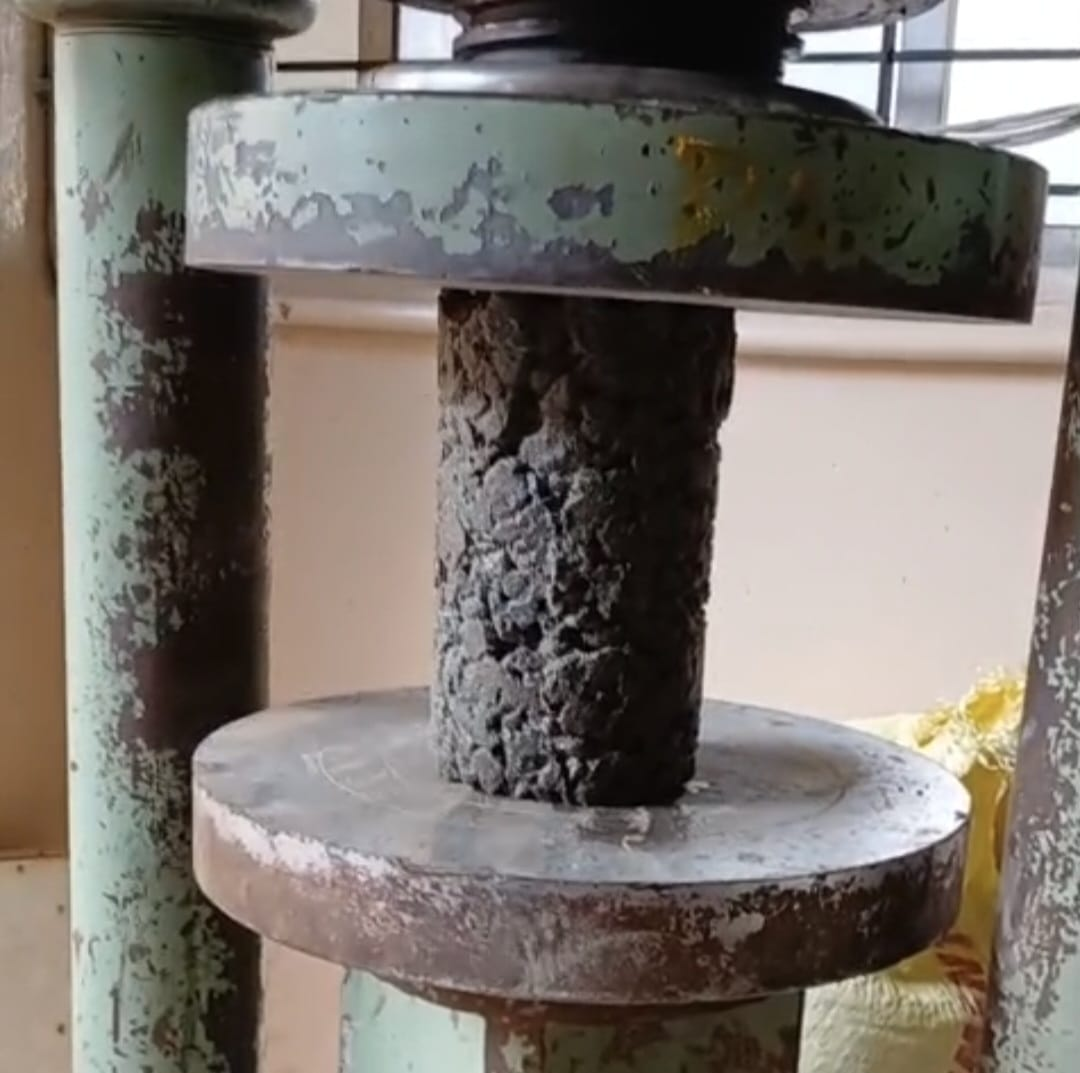
\includegraphics[scale=0.15]{compressive}
\end{figure}



\section{Results}

\begin{table}[htb]
    \begin{threeparttable}
        \caption{\textbf{Compressive and Tensile Strength}}
        \label{table:str-test}
        \setlength{\tabcolsep}{16.5pt}
        \def\arraystretch{1.5}%
        \begin{tabular}{ l r r r r }
            \hline
            & \multicolumn{2}{c}{Compressive, $Mpa$} & 
                \multicolumn{2}{c}{Tensile, $Mpa$} \\

            \cline{2-5}
            & \multicolumn{1}{c}{14} & \multicolumn{1}{c}{28} & 
                \multicolumn{1}{c}{14} & \multicolumn{1}{c}{28} \\

            \hline

            Batch 1 & 5.62 & 7.49  & 0.71 & 0.85 \\
            Batch 2 & 8.02 & 10.08 & 1.15 & 1.33 \\

            \hline
        \end{tabular} 
        \begin{tablenotes}
            \item Results of the compressive and tensile tests at the end of 
            14 and 28 days of curing.
        \end{tablenotes}
    \end{threeparttable}
\end{table}

\begin{table}[!htb]
    \begin{threeparttable}
        \caption{\textbf{Permeability}}
        \label{table:perm-test}
        \setlength{\tabcolsep}{16.5pt}
        \def\arraystretch{1.5}%
        \begin{tabular}{ l r r }
            \hline
            & \multicolumn{1}{c}{14} & \multicolumn{1}{c}{28} \\
            \hline

            Batch 1 & 2.90 & 1.73 \\ 
            Batch 2 & 1.93 & 1.15 \\

            \hline
        \end{tabular} 
        \begin{tablenotes}
            \item Results of the permeability ($mm/s$) tests at the end of 
            14 and 28 days of curing.
        \end{tablenotes}
    \end{threeparttable}
\end{table}

From the results given by table \ref{table:str-test}, it is apparent that the 
amount of water used in the mix greatly affects the final strength of the 
concrete, with the ones having a lower water-cement ratio outperforming the ones 
with a higher water-cement ratio.
The results of the permeability tests shown by table \ref{table:perm-test} imply
that the permeability decreases with the increase in the water content of the 
mix. 

\begin{figure}[h]
    \caption{Compressive Strength - Curing Period}
    \centering
    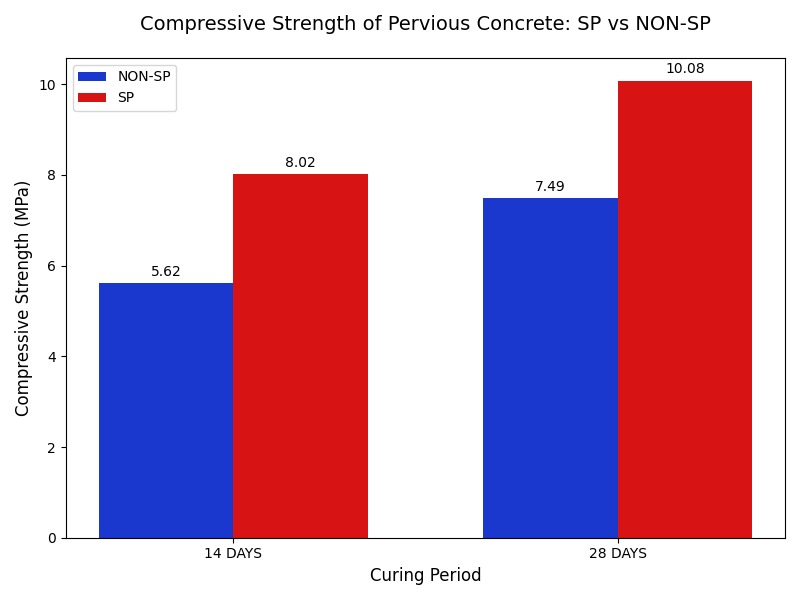
\includegraphics[scale=0.25]{comp-graph}
\end{figure}

\begin{figure}[h]
    \caption{Tensile Strength - Curing Period}
    \centering
    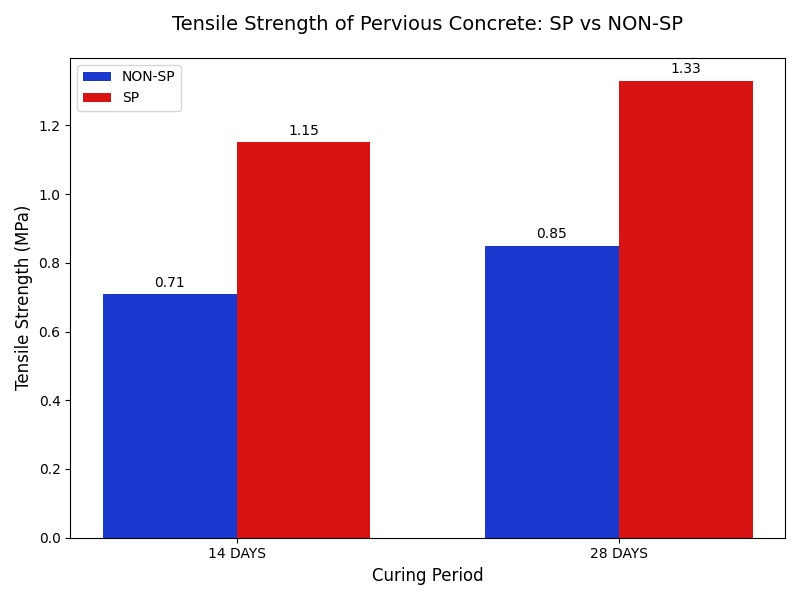
\includegraphics[scale=0.3]{tensile-graph}
\end{figure}

\begin{figure}[h]
    \caption{Plot of Permeability}
    \centering
    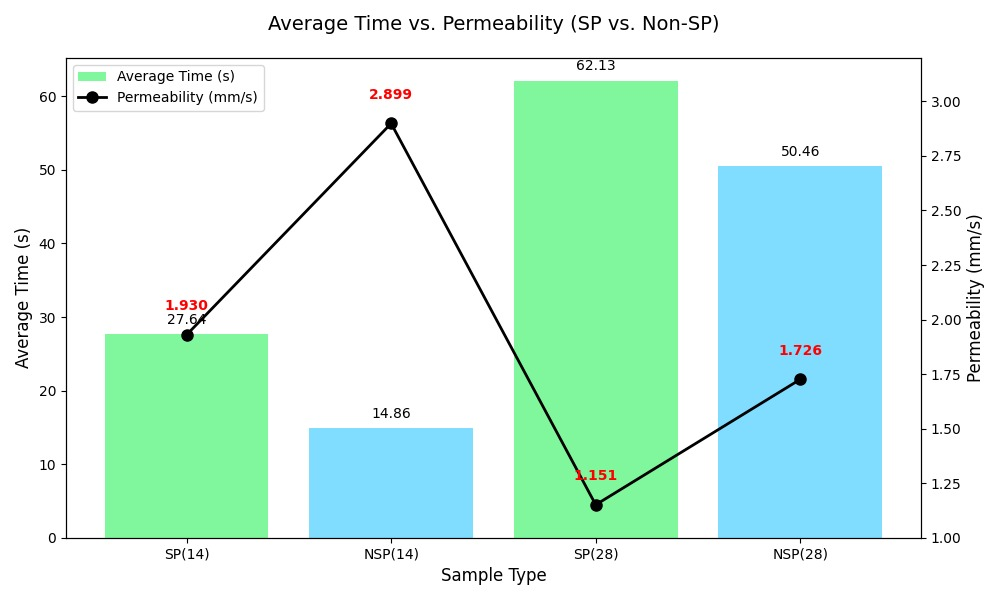
\includegraphics[scale=0.25]{perm-graph}
\end{figure}

\section{Conclusion}
Pervious concrete is shaping up to be a promising solution to the serious
environmental caused by the lack of water reclamation by the soil due to the
impervious nature of regular concrete, something that paves a large portion of
our land. However, the use of pervious concrete is, as of now, limited to
pavements and parking lots, due to its relatively low strength. 
From the tests of the two mixes, it can be seen that strength and permeability
are inversely proportional to each other, and that the optimal mix should find
a balance between the two. The mix proposed in this paper, although not by any
means optimal, comes somewhat close to achieving this, performing reasonably
well in permeability, as well as strength tests. 

\begin{thebibliography}{00}

\bibitem{b1} Chandrappa, A. K., \& Biligiri, K. P. (2016). Pervious concrete as
a sustainable pavement material–Research findings and future prospects:
A state-of-the-art review. Construction and building materials, 111, 262-274.

\bibitem{b2} Ali Toghroli, Peyman Mehrabi, Mahdi Shariati, Nguyen Thoi Trung,
Soheil Jahandari, Haleh Rasekh, Evaluating the use of recycled concrete
aggregate And pozzolanic additives in fibre-reinforced pervious concrete with
industrial and recycled fibres, Construction and Building Materials, Volume
252,2020,118997,ISSN 0950-0618 

\bibitem{b3} Leon Raj, J., \& Chockalingam, T. (2020). Strength and abrasion
    characteristics of pervious concrete. Road Materials and Pavement Design,
        21(8), 2180-2197.

\bibitem{b4} Khankhaje, E., Kim, T., Jang, H., Kim, C. S., Kim, J., \&
    Rafieizonooz, M.  (2024). A review of utilization of industrial waste
        materials as cement replacement in pervious concrete: An alternative
        approach to sustainable pervious concrete production. Heliyon, 10(4).

\end{thebibliography}


\EOD

\end{document}
